%=================================================================
% CSE 4345 — Big Data Analytics
% Week 11, Part 2: Seminal Research & Case Study
% Department of CSE, Premier University
%
% SEMINAL PAPERS:
%   Armbrust et al. (2020) — Delta Lake: High-Performance ACID
%   Table Storage over Cloud Object Stores. VLDB 2020.
%
%   Zaharia et al. (2021) — Lakehouse: A New Generation of Open
%   Platforms That Unify Data Warehousing and Advanced Analytics.
%   CIDR 2021.
%
%   Akidau et al. (2015) — The Dataflow Model: A Practical Approach
%   to Balancing Correctness, Latency, and Cost in Massive-Scale,
%   Unbounded, Out-of-Order Data Processing. PVLDB 2015.
%
% CASE STUDY:
%   Databricks Lakehouse Migration in Production —
%   From Lambda architecture to unified Lakehouse at enterprise scale;
%   lessons from Pinterest, Comcast, and Databricks' own platform.
%=================================================================

\documentclass[aspectratio=169,10pt]{beamer}

%---------- Packages ----------
\usepackage[utf8]{inputenc}
\usepackage[T1]{fontenc}
\usepackage{booktabs}
\usepackage{xcolor}
\usepackage{tikz}
\usetikzlibrary{shapes.geometric, positioning, arrows.meta,
                decorations.pathreplacing, calc}
\usepackage{amsmath}
\usepackage{graphicx}
\usepackage{multicol}
\usepackage{enumerate}
\usepackage{array}

%---------- Theme ----------
\usetheme{Madrid}

%---------- Premier University Color Identity ----------
\definecolor{PUNavy}{RGB}{10,36,99}
\definecolor{PUGold}{RGB}{197,151,37}
\definecolor{PULightBlue}{RGB}{210,228,255}
\definecolor{PUTeal}{RGB}{0,100,100}
\definecolor{PUGray}{RGB}{90,90,90}
\definecolor{PURed}{RGB}{160,30,30}
\definecolor{PUGreen}{RGB}{30,120,60}
\definecolor{PUPurple}{RGB}{90,30,120}
\definecolor{PUOrange}{RGB}{190,90,20}

\setbeamercolor{palette primary}{bg=PUNavy, fg=white}
\setbeamercolor{palette secondary}{bg=PUNavy!85, fg=white}
\setbeamercolor{palette tertiary}{bg=PUNavy!70, fg=white}
\setbeamercolor{palette quaternary}{bg=PUNavy, fg=white}
\setbeamercolor{structure}{fg=PUNavy}
\setbeamercolor{title}{bg=PUNavy, fg=PUGold}
\setbeamercolor{subtitle}{fg=white}
\setbeamercolor{frametitle}{bg=PUNavy, fg=PUGold}
\setbeamercolor{alerted text}{fg=PUGold!85!black}
\setbeamercolor{block title}{bg=PUNavy, fg=white}
\setbeamercolor{block body}{bg=PULightBlue!45}
\setbeamercolor{block title alerted}{bg=PUGold!80!black, fg=white}
\setbeamercolor{block body alerted}{bg=PUGold!12}
\setbeamercolor{block title example}{bg=PUTeal, fg=white}
\setbeamercolor{block body example}{bg=PUTeal!10}
\setbeamercolor{section in toc}{fg=PUNavy}
\setbeamercolor{itemize item}{fg=PUGold!80!black}
\setbeamercolor{itemize subitem}{fg=PUNavy!70}

\setbeamertemplate{navigation symbols}{}
\setbeamertemplate{itemize item}{\scriptsize\raise1.5pt\hbox{\textbullet}}
\setbeamertemplate{itemize subitem}{\scriptsize\raise1pt\hbox{--}}

%---------- Section separator ----------
\AtBeginSection[]{
  \begin{frame}[plain]
    \vfill
    \centering
    \begin{beamercolorbox}[sep=12pt,center,shadow=true,rounded=true]{block title}
      \usebeamerfont{title}\insertsectionhead\par
    \end{beamercolorbox}
    \vfill
  \end{frame}
}

%---------- Helper: citation box ----------
\newenvironment{paperbox}[1]{%
  \setbeamercolor{block title}{bg=PUNavy!90,fg=PUGold}
  \setbeamercolor{block body}{bg=PUNavy!6}
  \begin{block}{#1}}{%
  \end{block}}

%---------- Custom footline ----------
\setbeamertemplate{footline}{
  \leavevmode\hbox{%
    \begin{beamercolorbox}[wd=.333\paperwidth,ht=2.25ex,dp=1ex,center]{palette primary}
      \usebeamerfont{author in head/foot}\insertshortauthor
    \end{beamercolorbox}%
    \begin{beamercolorbox}[wd=.334\paperwidth,ht=2.25ex,dp=1ex,center]{palette secondary}
      \usebeamerfont{title in head/foot}\insertshorttitle
    \end{beamercolorbox}%
    \begin{beamercolorbox}[wd=.333\paperwidth,ht=2.25ex,dp=1ex,right]{palette primary}
      \usebeamerfont{date in head/foot}
      \insertframenumber{} / \inserttotalframenumber\hspace*{2ex}
    \end{beamercolorbox}}%
  \vskip0pt%
}

%---------- Title metadata ----------
\title[CSE 4345 \textbar{} Week 11, Part 2]{CSE 4345: Big Data Analytics}
\subtitle{Week 11, Part 2 \textemdash\ Seminal Research \& Case Study}
\author[Dept.\ of CSE]{Department of Computer Science \& Engineering\\[4pt]
       \small Premier University, Chittagong}
\institute{}
\date{Semester 2026}

%=================================================================
\begin{document}
%=================================================================

\begin{frame}
  \titlepage
\end{frame}

%----------------------------------------------------------------
\begin{frame}{Part 2 Overview — Week 11 (Course Finale)}
  \begin{columns}[T]
    \column{0.46\textwidth}
      \begin{block}{Today's Agenda}
        \tableofcontents
      \end{block}
    \column{0.51\textwidth}
      \begin{exampleblock}{Seminal Papers Covered}
        \begin{enumerate}
          \item Armbrust et al. (2020).
                \textit{Delta Lake: High-Performance ACID Table
                Storage over Cloud Object Stores.} VLDB 2020.
          \item Armbrust, Ghodsi, Xin \& Zaharia (2021).
                \textit{Lakehouse: A New Generation of Open Platforms
                That Unify Data Warehousing and Advanced Analytics.}
                CIDR 2021.
          \item Akidau et al. (2015).
                \textit{The Dataflow Model.} PVLDB 2015.
        \end{enumerate}
      \end{exampleblock}
      \vspace{5pt}
      \begin{alertblock}{Case Study}
        \textbf{Enterprise Lakehouse Migration} — how Pinterest
        (300+ PB), Comcast (100 TB/day) and Databricks replaced
        their Lambda-architecture stacks with a unified Lakehouse,
        cutting pipeline code by 70\% and storage cost by 60\%.
      \end{alertblock}
      \vspace{4pt}
      \begin{block}{CLO Addressed}
        \textbf{CLO4} — Synthesize the full course stack through
        emerging Lakehouse and unified streaming architectures\\
        \textbf{PLO(c,d,f)}
      \end{block}
  \end{columns}
\end{frame}

%================================================================
\section{Paper 1 — Armbrust et al.\ (2020): Delta Lake}
%================================================================

%----------------------------------------------------------------
\begin{frame}{Evolution of Analytics Architectures}
  \begin{center}
  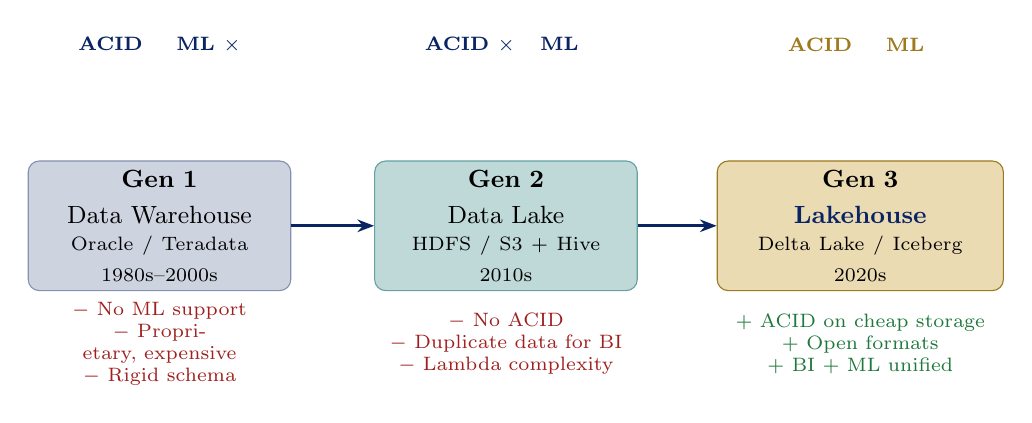
\begin{tikzpicture}[
      gen/.style={rectangle, rounded corners=4pt,
                  minimum width=3.3cm, minimum height=1.6cm,
                  text width=3.1cm, align=center, font=\small},
      arr/.style={-{Stealth[length=6pt]}, draw=PUNavy, very thick}
    ]
    % Generation 1 — Data Warehouse
    \node[gen, fill=PUNavy!20, draw=PUNavy!50]
          (dw) at (0, 0) {%
            \textbf{Gen 1}\\[2pt]
            Data Warehouse\\[2pt]
            \scriptsize Oracle / Teradata\\
            \scriptsize 1980s–2000s};

    % Generation 2 — Data Lake
    \node[gen, fill=PUTeal!25, draw=PUTeal!60]
          (dl) at (4.4, 0) {%
            \textbf{Gen 2}\\[2pt]
            Data Lake\\[2pt]
            \scriptsize HDFS / S3 + Hive\\
            \scriptsize 2010s};

    % Generation 3 — Lakehouse
    \node[gen, fill=PUGold!35, draw=PUGold!80!black,
          minimum width=3.6cm, minimum height=1.6cm,
          text width=3.4cm]
          (lh) at (8.9, 0) {%
            \textbf{Gen 3}\\[2pt]
            \textcolor{PUNavy}{\textbf{Lakehouse}}\\[2pt]
            \scriptsize Delta Lake / Iceberg\\
            \scriptsize 2020s};

    \draw[arr] (dw) -- (dl);
    \draw[arr] (dl) -- (lh);

    % Problems of each generation — below
    \node[font=\scriptsize, text=PURed, text width=3.0cm, align=center]
          at (0, -1.5) {$-$ No ML support\\$-$ Proprietary, expensive\\$-$ Rigid schema};
    \node[font=\scriptsize, text=PURed, text width=3.1cm, align=center]
          at (4.4, -1.5) {$-$ No ACID\\$-$ Duplicate data for BI\\$-$ Lambda complexity};
    \node[font=\scriptsize, text=PUGreen, text width=3.4cm, align=center]
          at (8.9, -1.5) {$+$ ACID on cheap storage\\$+$ Open formats\\$+$ BI + ML unified};

    % Feature comparison row
    \node[font=\scriptsize\bfseries, text=PUNavy] at (0,   2.3)
          {ACID $\checkmark$ \ \ ML $\times$};
    \node[font=\scriptsize\bfseries, text=PUNavy] at (4.4, 2.3)
          {ACID $\times$ \ \ ML $\checkmark$};
    \node[font=\scriptsize\bfseries, text=PUGold!80!black] at (8.9,2.3)
          {ACID $\checkmark$ \ \ ML $\checkmark$};
  \end{tikzpicture}
  \end{center}
  \vspace{6pt}
  \begin{alertblock}{The Fundamental Problem (2015--2020)}
    Enterprises ran \textbf{two separate systems}: a data lake (S3 + Spark)
    for ML workloads and a data warehouse (Redshift / Snowflake) for BI.
    This doubled ETL pipelines, storage cost, and data consistency risk.
    Delta Lake was built to eliminate this split.
  \end{alertblock}
\end{frame}

%----------------------------------------------------------------
\begin{frame}{Delta Lake: Publication Context \& Core Mechanism}
  \begin{columns}[T]
    \column{0.52\textwidth}
      \begin{paperbox}{Full Citation}
        Armbrust, M., Das, T., Willis, J., Zhu, S., Condie, T.,
        Zheng, S., Xin, R., \& Zaharia, M. (2020).
        \textbf{Delta Lake: High-Performance ACID Table Storage
        over Cloud Object Stores.}
        \textit{Proceedings of the VLDB Endowment, 13}(12),
        3411--3424.\\[5pt]
        \textbf{Venue:} VLDB 2020 — Rank A* (CORE)\\
        \textbf{Organization:} Databricks / Apache Software Foundation\\
        \textbf{Open source:} Apache License 2.0 at
        \texttt{delta.io}; native to Apache Spark
      \end{paperbox}
      \vspace{5pt}
      \begin{block}{The Core Insight}
        Cloud object stores (S3, Azure Blob, GCS) are
        \textbf{not file systems}: they lack atomic renames,
        directory listings are inconsistent under concurrent writes,
        and there is no native locking mechanism.\\[4pt]
        Delta Lake solves this with a \textbf{transaction log}
        (the \emph{Delta Log}) stored as a series of JSON files
        inside the table directory — implementing
        \textbf{Optimistic Concurrency Control} (OCC) on top of
        eventually-consistent object storage.
      \end{block}

    \column{0.45\textwidth}
      \begin{center}
      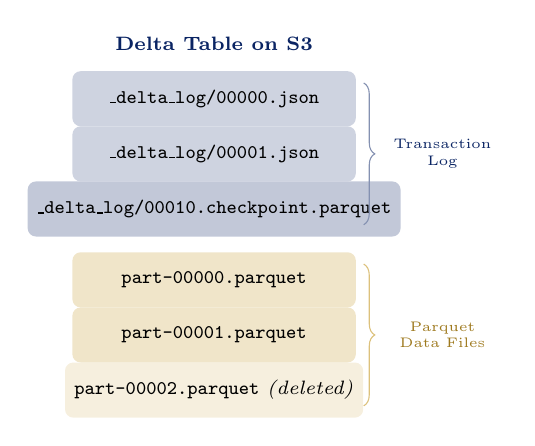
\begin{tikzpicture}[
          bx/.style={rectangle, rounded corners=3pt,
                     minimum width=3.6cm, minimum height=0.7cm,
                     align=center, font=\scriptsize},
          arr/.style={-{Stealth[length=4pt]}, draw=PUNavy, thick}
        ]
        \node[font=\scriptsize\bfseries, text=PUNavy] at (0, 5.2)
              {Delta Table on S3};

        \node[bx, fill=PUNavy!20] (log0)  at (0, 4.5)
              {\texttt{\_delta\_log/00000.json}};
        \node[bx, fill=PUNavy!20] (log1)  at (0, 3.8)
              {\texttt{\_delta\_log/00001.json}};
        \node[bx, fill=PUNavy!25] (ckpt)  at (0, 3.1)
              {\texttt{\_delta\_log/00010.checkpoint.parquet}};
        \node[bx, fill=PUGold!25] (data1) at (0, 2.2)
              {\texttt{part-00000.parquet}};
        \node[bx, fill=PUGold!25] (data2) at (0, 1.5)
              {\texttt{part-00001.parquet}};
        \node[bx, fill=PUGold!15] (data3) at (0, 0.8)
              {\texttt{part-00002.parquet} \textit{(deleted)}};

        \draw[decorate, decoration={brace,amplitude=4pt},
              draw=PUNavy!50]
              (1.9,4.7) -- (1.9,2.9)
              node[midway, right=5pt, font=\tiny, text=PUNavy,
                   align=center, text width=1.4cm]
              {Transaction\\Log};
        \draw[decorate, decoration={brace,amplitude=4pt},
              draw=PUGold!60]
              (1.9,2.4) -- (1.9,0.6)
              node[midway, right=5pt, font=\tiny, text=PUGold!80!black,
                   align=center, text width=1.4cm]
              {Parquet\\Data Files};
      \end{tikzpicture}
      \end{center}
  \end{columns}
\end{frame}

%----------------------------------------------------------------
\begin{frame}{Technical Contribution 1 — ACID via the Delta Log}
  \begin{columns}[T]
    \column{0.50\textwidth}
      \begin{block}{How ACID is Achieved}
        Each \textbf{transaction} (insert, update, delete, merge)
        appends exactly one JSON entry to the Delta Log recording:
        \begin{itemize}
          \item \textbf{Add} actions: new Parquet files written
          \item \textbf{Remove} actions: old files logically deleted
          \item \textbf{Metadata} changes: schema updates, config
          \item \textbf{Protocol} version: minimum reader/writer version
        \end{itemize}
        \textbf{Atomicity}: a transaction either appends its log entry
        completely or not at all (S3 object PUT is atomic).\\[4pt]
        \textbf{Isolation}: OCC — concurrent writers try to append
        the same log entry number; only one succeeds (S3 conditional
        PUT); the loser retries or fails.\\[4pt]
        \textbf{Consistency}: the Delta Log is the single source of
        truth for which files are valid; readers never see partial writes.\\[4pt]
        \textbf{Durability}: all committed log entries persist in
        S3 indefinitely — no in-memory state.
      \end{block}

    \column{0.47\textwidth}
      \begin{block}{Time Travel \& Schema Features}
        \textbf{Time travel (data versioning):}
        Because every version of the table is preserved in the
        log, Delta Lake supports reading any past snapshot:
        \begin{itemize}
          \item \texttt{VERSION AS OF 42}: read table at version 42
          \item \texttt{TIMESTAMP AS OF '2024-01-01'}:
                point-in-time query
          \item Enables \textbf{audit trails}, \textbf{rollback},
                and \textbf{reproducible ML experiments}
                (lock a training dataset to a specific version)
        \end{itemize}
      \end{block}
      \vspace{4pt}
      \begin{exampleblock}{Schema Enforcement \& Evolution}
        \begin{itemize}
          \item \textbf{Schema enforcement}: rejects writes that
                don't match the declared schema —
                eliminates ``data swamp'' corruption
          \item \textbf{Schema evolution}: controlled addition of
                new columns via \texttt{MERGE SCHEMA} option
          \item \textbf{Z-ordering}: co-locates related data in
                Parquet files for multi-column data skipping —
                queries with \texttt{WHERE} on multiple columns
                skip up to 95\% of files
        \end{itemize}
      \end{exampleblock}
  \end{columns}
\end{frame}

%================================================================
\section{Paper 2 — Zaharia et al.\ (2021): Lakehouse}
%================================================================

%----------------------------------------------------------------
\begin{frame}{Lakehouse: Publication Context \& Architecture}
  \begin{columns}[T]
    \column{0.52\textwidth}
      \begin{paperbox}{Full Citation}
        Armbrust, M., Ghodsi, A., Xin, R., \& Zaharia, M. (2021).
        \textbf{Lakehouse: A New Generation of Open Platforms
        That Unify Data Warehousing and Advanced Analytics.}
        \textit{11th Annual Conference on Innovative Data Systems
        Research (CIDR 2021)}.\\[5pt]
        \textbf{Venue:} CIDR 2021 — premier systems vision paper venue\\
        \textbf{Organization:} Databricks\\
        \textbf{Significance:} First formal architectural definition
        of the Lakehouse paradigm; cited by Snowflake, Google
        BigLake, and AWS Lake Formation design documents
      \end{paperbox}
      \vspace{5pt}
      \begin{block}{The Lakehouse Definition}
        A Lakehouse is a data management system that combines:
        \begin{enumerate}
          \item \textbf{Cheap, open storage} (S3, ADLS, GCS) in
                open formats (Parquet, ORC) — like a data lake
          \item \textbf{Metadata \& governance layer}
                (Delta Lake / Iceberg / Hudi) providing ACID,
                schema, and versioning — like a data warehouse
          \item \textbf{Unified query engine} (Spark SQL) serving
                both BI dashboards and ML training on the
                \emph{same} data — no ETL copy needed
        \end{enumerate}
      \end{block}

    \column{0.45\textwidth}
      \begin{center}
      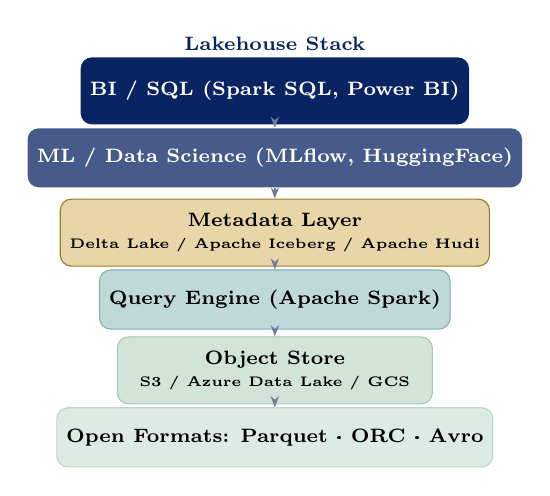
\begin{tikzpicture}[
          bx/.style={rectangle, rounded corners=4pt,
                     minimum width=4.0cm, minimum height=0.75cm,
                     align=center, font=\scriptsize\bfseries},
          arr/.style={-{Stealth[length=4pt]}, draw=PUNavy!60, thick}
        ]
        \node[font=\scriptsize\bfseries, text=PUNavy] at (0, 5.6)
              {Lakehouse Stack};

        \node[bx, fill=PUNavy, text=white, minimum height=0.85cm]
              (bi)   at (0, 5.0) {BI / SQL (Spark SQL, Power BI)};
        \node[bx, fill=PUNavy!75, text=white]
              (ml)   at (0, 4.15) {ML / Data Science (MLflow, HuggingFace)};

        \node[bx, fill=PUGold!40, draw=PUGold!80!black, minimum height=0.85cm]
              (meta) at (0, 3.2)
              {Metadata Layer\\{\tiny Delta Lake / Apache Iceberg / Apache Hudi}};

        \node[bx, fill=PUTeal!25, draw=PUTeal!50]
              (eng)  at (0, 2.35) {Query Engine (Apache Spark)};

        \node[bx, fill=PUGreen!20, draw=PUGreen!40, minimum height=0.85cm]
              (stor) at (0, 1.45)
              {Object Store\\{\tiny S3 / Azure Data Lake / GCS}};
        \node[bx, fill=PUGreen!15, draw=PUGreen!30]
              (fmt)  at (0, 0.6)  {Open Formats: Parquet · ORC · Avro};

        \foreach \a/\b in {bi/ml, ml/meta, meta/eng, eng/stor, stor/fmt}{
          \draw[arr] (\a) -- (\b);
        }
      \end{tikzpicture}
      \end{center}
  \end{columns}
\end{frame}

%----------------------------------------------------------------
\begin{frame}{Lakehouse vs.\ Data Warehouse vs.\ Data Lake}
  \begin{columns}[T]
    \column{0.55\textwidth}
      \renewcommand{\arraystretch}{1.3}
      \begin{tabular}{@{}p{2.5cm}p{2.0cm}p{2.0cm}p{2.0cm}@{}}
        \toprule
        \textbf{Feature} & \textbf{DW} & \textbf{Lake} & \textbf{Lakehouse} \\
        \midrule
        Storage cost    & High (proprietary) & Low (S3)    & Low (S3) \\
        Open format     & No          & Yes           & Yes \\
        ACID txns       & Yes         & No            & Yes \\
        Schema enforce. & Yes         & No            & Yes \\
        BI / SQL        & Yes         & Partial       & Yes \\
        ML / streaming  & No          & Yes           & Yes \\
        Time travel     & No          & No            & Yes \\
        Single copy     & No (ETL copy) & N/A         & \textbf{Yes} \\
        \bottomrule
      \end{tabular}
      \vspace{8pt}
      \begin{alertblock}{The ``No ETL Copy'' Advantage}
        Traditional stacks copy data from lake to warehouse for BI —
        doubling storage cost and introducing consistency lag
        (warehouse data is always hours behind the lake).
        The Lakehouse serves both BI and ML from a single
        ACID-consistent copy: \textbf{one truth, two workloads}.
      \end{alertblock}

    \column{0.42\textwidth}
      \begin{block}{Competing Open Table Formats}
        The Lakehouse paper catalysed an ecosystem of
        open metadata formats:
        \begin{itemize}
          \item \textbf{Delta Lake} (Databricks / Apache): native
                Spark; strongest adoption; Z-ordering; CDC support
          \item \textbf{Apache Iceberg} (Netflix origin):
                vendor-neutral; hidden partitioning; partition
                evolution; Flink + Trino + Spark support
          \item \textbf{Apache Hudi} (Uber origin): record-level
                upserts; incremental processing; CDC out-of-box
        \end{itemize}
        \textbf{2023--24 convergence:} Delta and Iceberg are
        adopting a shared \textbf{UniForm} metadata standard
        so a single table can be read by both engines simultaneously.
      \end{block}
  \end{columns}
\end{frame}

%================================================================
\section{Paper 3 — Akidau et al.\ (2015): The Dataflow Model}
%================================================================

%----------------------------------------------------------------
\begin{frame}{Dataflow Model: Unifying Batch and Stream Processing}
  \begin{columns}[T]
    \column{0.52\textwidth}
      \begin{paperbox}{Full Citation}
        Akidau, T., Bradshaw, R., Chambers, C., et al. (2015).
        \textbf{The Dataflow Model: A Practical Approach to
        Balancing Correctness, Latency, and Cost in
        Massive-Scale, Unbounded, Out-of-Order Data Processing.}
        \textit{Proceedings of the VLDB Endowment, 8}(12),
        1792--1803.\\[5pt]
        \textbf{Venue:} PVLDB 2015 — VLDB Best Paper\\
        \textbf{Organization:} Google\\
        \textbf{Open source:} Led to \textbf{Apache Beam}
        (2016); runs on Spark, Flink, Google Dataflow backends
      \end{paperbox}
      \vspace{5pt}
      \begin{block}{The Four Questions (The ``Four Ws'')}
        Any data processing pipeline can be described by:
        \begin{enumerate}
          \item \textbf{What} results are computed?
                (transformations: map, groupBy, join)
          \item \textbf{Where} in \emph{event time}?
                (windowing: tumbling, sliding, session)
          \item \textbf{When} in \emph{processing time}?
                (triggers: watermark, periodic, count)
          \item \textbf{How} do refinements relate?
                (accumulation: discard, accumulate, retract)
        \end{enumerate}
        This model subsumes batch (unbounded window, watermark at EOF)
        as a special case of streaming — eliminating the Lambda
        architecture's dual code path.
      \end{block}

    \column{0.45\textwidth}
      \begin{center}
      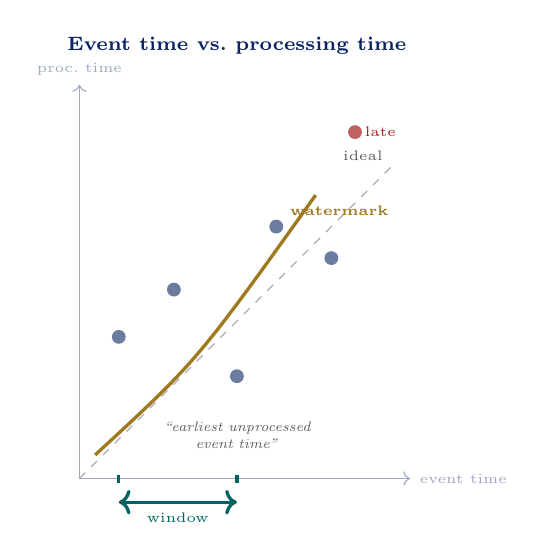
\begin{tikzpicture}[
          wbox/.style={rectangle, rounded corners=3pt,
                       minimum width=3.2cm, minimum height=0.8cm,
                       align=center, font=\scriptsize\bfseries}
        ]
        \node[font=\scriptsize\bfseries, text=PUNavy] at (0, 5.5)
              {Event time vs.\ processing time};

        % Event time axis
        \draw[PUNavy!40, ->] (-2.0, 0.0) -- (2.2, 0.0)
              node[right, font=\tiny] {event time};
        \draw[PUNavy!40, ->] (-2.0, 0.0) -- (-2.0, 5.0)
              node[above, font=\tiny] {proc.\ time};

        % Ideal diagonal
        \draw[PUGray!50, dashed, thin] (-2.0, 0.0) -- (2.0, 4.0);
        \node[font=\tiny, text=PUGray] at (1.6, 4.1) {ideal};

        % Real event-time skew dots
        \fill[PUNavy!60] (-1.5, 1.8) circle (2.5pt);
        \fill[PUNavy!60] (-0.8, 2.4) circle (2.5pt);
        \fill[PUNavy!60] (0.0,  1.3) circle (2.5pt);
        \fill[PUNavy!60] (0.5,  3.2) circle (2.5pt);
        \fill[PUNavy!60] (1.2,  2.8) circle (2.5pt);
        \fill[PURed!70]  (1.5,  4.4) circle (2.5pt)
              node[right, font=\tiny, text=PURed] {late};

        % Watermark line
        \draw[PUGold!80!black, very thick]
              (-1.8, 0.3) .. controls (-0.5, 1.5) .. (1.0, 3.6);
        \node[font=\tiny\bfseries, text=PUGold!80!black]
              at (1.3, 3.4) {watermark};
        \node[font=\tiny\itshape, text=PUGray, text width=2.0cm,
              align=center] at (0, 0.55)
              {``earliest unprocessed\\event time''};

        % Window bracket
        \draw[PUTeal, very thick]
              (-1.5, -0.05) -- (-1.5, 0.05);
        \draw[PUTeal, very thick]
              (0.0, -0.05) -- (0.0, 0.05);
        \draw[PUTeal, <->, very thick]
              (-1.5, -0.3) -- (0.0, -0.3)
              node[midway, below, font=\tiny] {window};
      \end{tikzpicture}
      \end{center}
      \begin{exampleblock}{Apache Beam Impact}
        \scriptsize
        The same Beam pipeline code runs on Spark (batch),
        Flink (stream), or Google Dataflow (managed) —
        write once, run anywhere.
        Adopted by Google, LinkedIn, PayPal, and Spotify.
      \end{exampleblock}
  \end{columns}
\end{frame}

%================================================================
\section{Case Study — Enterprise Lakehouse Migration in Production}
%================================================================

%----------------------------------------------------------------
\begin{frame}{From Lambda Architecture to Lakehouse}
  \begin{columns}[T]
    \column{0.52\textwidth}
      \begin{block}{The Problem: Lambda at Scale}
        By 2018--2020, large enterprises running Lambda architecture
        faced compounding pain:
        \begin{itemize}
          \item \textbf{Pinterest (300+ PB):}
                two code paths (Spark batch + Flink stream) for
                every metric — engineers spent 40\% of time keeping
                them in sync
          \item \textbf{Comcast (100 TB/day):}
                data copied from S3 (lake) to Redshift (DWH) nightly,
                creating a 12-hour data freshness gap for analysts
          \item \textbf{Generic pattern:}
                3--5 ETL pipelines per business metric;
                data quality issues discovered hours after ingestion;
                ML feature store diverged from BI tables
        \end{itemize}
      \end{block}
      \vspace{4pt}
      \begin{alertblock}{The Migration Goal}
        Replace the Lambda stack (HDFS/S3 lake + Redshift/Hive DWH)
        with a single Lakehouse (Delta Lake on S3 + Spark SQL),
        serving both streaming ingestion and interactive BI from
        one ACID table — no ETL copy, no dual code path.
      \end{alertblock}

    \column{0.45\textwidth}
      \begin{center}
      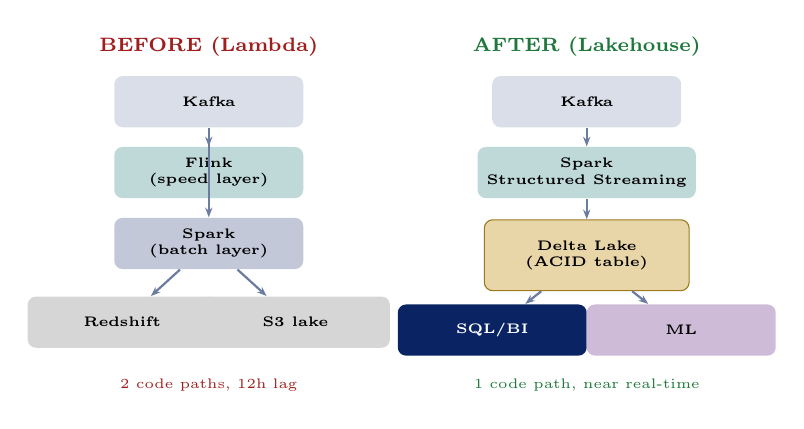
\begin{tikzpicture}[
          bx/.style={rectangle, rounded corners=3pt,
                     minimum width=2.4cm, minimum height=0.65cm,
                     align=center, font=\tiny\bfseries},
          arr/.style={-{Stealth[length=3.5pt]}, draw=PUNavy!60, thick}
        ]
        % BEFORE
        \node[font=\scriptsize\bfseries, text=PURed] at (-1.5, 5.2)
              {BEFORE (Lambda)};
        \node[bx, fill=PUNavy!15] (kfk1) at (-1.5, 4.5) {Kafka};
        \node[bx, fill=PUTeal!25]  (spd)  at (-1.5, 3.6) {Flink\\(speed layer)};
        \node[bx, fill=PUNavy!25]  (bat)  at (-1.5, 2.7) {Spark\\(batch layer)};
        \node[bx, fill=PUGray!25]  (dw1)  at (-2.6, 1.7) {Redshift};
        \node[bx, fill=PUGray!25]  (lk1)  at (-0.4, 1.7) {S3 lake};
        \draw[arr] (kfk1)--(spd); \draw[arr] (kfk1)--(bat);
        \draw[arr] (bat)--(dw1); \draw[arr] (bat)--(lk1);
        \node[font=\tiny, text=PURed] at (-1.5, 0.9)
              {2 code paths, 12h lag};

        % AFTER
        \node[font=\scriptsize\bfseries, text=PUGreen] at (3.3, 5.2)
              {AFTER (Lakehouse)};
        \node[bx, fill=PUNavy!15] (kfk2) at (3.3, 4.5) {Kafka};
        \node[bx, fill=PUTeal!25]  (ss)   at (3.3, 3.6) {Spark\\Structured Streaming};
        \node[bx, fill=PUGold!40, draw=PUGold!80!black,
              minimum width=2.6cm, minimum height=0.9cm]
              (lh)   at (3.3, 2.55) {Delta Lake\\(ACID table)};
        \node[bx, fill=PUNavy, text=white] (bi2) at (2.1, 1.6) {SQL/BI};
        \node[bx, fill=PUPurple!30] (ml2) at (4.5, 1.6) {ML};
        \draw[arr] (kfk2)--(ss); \draw[arr] (ss)--(lh);
        \draw[arr] (lh)--(bi2); \draw[arr] (lh)--(ml2);
        \node[font=\tiny, text=PUGreen] at (3.3, 0.9)
              {1 code path, near real-time};
      \end{tikzpicture}
      \end{center}
  \end{columns}
\end{frame}

%----------------------------------------------------------------
\begin{frame}{Measured Outcomes \& Key Lessons}
  \begin{columns}[T]
    \column{0.52\textwidth}
      \begin{block}{Production Results (Composite from Public Reports)}
        \renewcommand{\arraystretch}{1.25}
        \begin{tabular}{@{}p{4.0cm}p{1.8cm}p{1.8cm}@{}}
          \toprule
          \textbf{Metric} & \textbf{Before} & \textbf{After} \\
          \midrule
          ETL pipeline count (per metric) & 3--5 jobs & 1 job \\
          Data freshness (BI)             & 12 hours  & $<$15 min \\
          Storage cost (per TB)           & \$230 DWH & \$23 S3 \\
          ML experiment reproducibility   & Manual    & Versioned \\
          Failed jobs due to bad schema   & Weekly    & Blocked at ingest \\
          Analyst query wait (P95)        & 8 min     & 45 sec \\
          \bottomrule
        \end{tabular}
        \vspace{4pt}
        \small
        \textbf{Sources:} Pinterest Engineering Blog (2021);
        Comcast BDTC Talk (2020); Databricks Lakehouse Summit (2022)
      \end{block}

    \column{0.45\textwidth}
      \begin{block}{Key Lessons Learned}
        \begin{enumerate}
          \item \textbf{Migration, not big-bang replacement}:
                Lakehouse teams migrated one table at a time,
                running Delta Lake and legacy DWH in parallel
                until each table validated — zero downtime
          \item \textbf{Schema enforcement first}:
                teams that enabled schema enforcement on day 1
                found and fixed 90\% of data quality bugs within
                the first week; teams that deferred it spent
                months debugging corrupted tables
          \item \textbf{Time travel as an audit tool}:
                Compliance teams adopted \texttt{VERSION AS OF}
                queries to answer ``what did the table look like
                on December 31?'' — eliminating manual snapshot exports
          \item \textbf{Z-ordering beats blanket partitioning}:
                traditional Hive partitioning on a single column
                (e.g., \texttt{date}) failed for multi-column
                filters; Z-ordering on \texttt{(user\_id, date)}
                reduced scanned files by 80\%
        \end{enumerate}
      \end{block}
  \end{columns}
\end{frame}

%----------------------------------------------------------------
\begin{frame}{Discussion Questions — Course Synthesis}
  \begin{columns}[T]
    \column{0.52\textwidth}
      \begin{block}{Technical Questions \textmd{\tiny (CLO4 — Apply/Analyse)}}
        \begin{enumerate}
          \item \textbf{ACID on S3}: Delta Lake achieves atomicity
                by treating S3 object PUT as atomic.
                Identify two scenarios where this guarantee can
                still break (hint: S3 eventual consistency pre-2020,
                multi-region buckets) and explain how Delta Lake
                mitigates them.
                \textit{[CLO4 — Analyse]}

          \item \textbf{Dataflow Four Ws}: A payment fraud detection
                pipeline receives transactions with a 30-second
                event-time lag (mobile app buffers).
                Define the four Ws for a tumbling 5-minute window
                that emits results when the watermark passes the
                window end AND allows late arrivals up to 2 minutes.
                Which Apache Beam trigger policy would you use?
                \textit{[CLO4 — Apply]}

          \item \textbf{Lakehouse vs.\ Snowflake}: Your CTO argues
                that a managed cloud warehouse (Snowflake) is simpler
                than a self-managed Delta Lake Lakehouse.
                Under what conditions is the CTO right?
                When would you insist on the Lakehouse approach?
                \textit{[CLO4 — Evaluate]}
        \end{enumerate}
      \end{block}

    \column{0.45\textwidth}
      \begin{alertblock}{Capstone Design Question \textmd{\tiny (CLO4 — Design)}}
        \textbf{Design a Lakehouse for a Bangladeshi national health
        analytics platform:}
        \begin{itemize}
          \item \textbf{Sources}: 300 hospitals (HL7 FHIR), pharmacy
                chains, national disease registry (CDC-style)
          \item \textbf{Requirements}: HIPAA-equivalent privacy;
                near-real-time dengue/cholera alert generation;
                long-term epidemiology research access; Prophet-based
                seasonal disease forecasting
        \end{itemize}
        \vspace{4pt}
        Specify:
        \begin{enumerate}
          \item Ingestion layer (Kafka topics, connectors)
          \item Storage layer (Delta Lake table design, partitioning)
          \item Query layer (Spark SQL, access control)
          \item ML layer (MLflow experiment tracking)
          \item Governance (schema enforcement, time travel for audit)
        \end{enumerate}
        \textit{[CLO4 — Design, 300 words]}
      \end{alertblock}
  \end{columns}
\end{frame}

%================================================================
\section{Live Exercise}
%================================================================

%----------------------------------------------------------------
\begin{frame}[fragile]{Live Exercise — Delta Lake ACID Operations}
  \begin{columns}[T]
    \column{0.48\textwidth}
      \begin{block}{Task (30 minutes, pairs)}
        Explore Delta Lake's core ACID features using
        \textbf{PySpark + delta-spark} locally:
        \begin{enumerate}\setlength\itemsep{1pt}
          \item Write a Parquet-format DataFrame as a Delta table.
          \item Append new rows (atomic transaction).
          \item Perform an \textbf{UPDATE} (changes logged in
                Delta Log).
          \item Read the table \textbf{at version 0} to verify
                time travel.
          \item Run \texttt{DESCRIBE HISTORY} to inspect the
                full transaction log.
          \item Break schema enforcement: try inserting a row
                with a wrong column type and observe the error.
        \end{enumerate}
      \end{block}
      \vspace{4pt}
      \begin{exampleblock}{Install}
        \scriptsize
        \texttt{pip install delta-spark pyspark}
      \end{exampleblock}

    \column{0.49\textwidth}
      \begin{exampleblock}{Python Skeleton}
        \scriptsize
        \begin{verbatim}
from pyspark.sql import SparkSession
from delta import configure_spark_with_delta_pip

builder = (SparkSession.builder
           .appName("DeltaDemo")
           .config("spark.sql.extensions",
             "io.delta.sql.DeltaSparkSessionExtension")
           .config("spark.sql.catalog.spark_catalog",
             "org.apache.spark.sql.delta.catalog"
             ".DeltaCatalog"))

spark = configure_spark_with_delta_pip(
          builder).getOrCreate()

# -- Create Delta table --
df = spark.createDataFrame([
  (1,"Alice",30),(2,"Bob",25)],
  ["id","name","age"])
df.write.format("delta").save("/tmp/demo_table")

# -- Append (new transaction) --
df2 = spark.createDataFrame([
  (3,"Carol",35)], ["id","name","age"])
df2.write.format("delta").mode("append")\
         .save("/tmp/demo_table")

# -- Update (SQL) --
spark.sql("""UPDATE delta.`/tmp/demo_table`
             SET age = 31 WHERE name = 'Alice'""")

# -- Time travel: read version 0 --
v0 = (spark.read.format("delta")
      .option("versionAsOf", 0)
      .load("/tmp/demo_table"))
v0.show()  # Alice age=30, Bob age=25

# -- Transaction history --
spark.sql("""DESCRIBE HISTORY
             delta.`/tmp/demo_table`""").show()
        \end{verbatim}
      \end{exampleblock}
  \end{columns}
\end{frame}

%================================================================
\section*{References}
%================================================================

%----------------------------------------------------------------
\begin{frame}{References}
  \begin{block}{Seminal Papers}
    \begin{itemize}
      \item Armbrust, M., et al. (2020). Delta Lake: High-performance
            ACID table storage over cloud object stores.
            \textit{PVLDB, 13}(12), 3411--3424.
      \item Armbrust, M., Ghodsi, A., Xin, R., \& Zaharia, M. (2021).
            Lakehouse: A new generation of open platforms that unify
            data warehousing and advanced analytics.
            \textit{CIDR 2021}.
      \item Akidau, T., et al. (2015). The Dataflow model.
            \textit{PVLDB, 8}(12), 1792--1803.
    \end{itemize}
  \end{block}
  \vspace{4pt}
  \begin{block}{Textbooks \textmd{[TW], [SA], [TE]}}
    \begin{itemize}
      \item \textbf{[TW]} White, T. (2015).
            \textit{Hadoop: The Definitive Guide}, 4th ed. O'Reilly.
      \item \textbf{[SA]} Acharya, S., \& Chellappan, S. (2015).
            \textit{Big Data and Analytics} (Ch.~12). Wiley.
      \item \textbf{[TE]} Erl, T., et al. (2016).
            \textit{Big Data Fundamentals} (Ch.~13). Prentice Hall.
    \end{itemize}
  \end{block}
  \vspace{4pt}
  \begin{block}{Case Study Sources}
    \begin{itemize}
      \item Pinterest Engineering Blog (2021). Building Pinterest's
            new wide column storage system.
      \item Databricks (2022). State of Data + AI Report.
            Lakehouse migration patterns and benchmarks.
      \item Kleppmann, M. (2017). \textit{Designing Data-Intensive
            Applications}. O'Reilly (Ch.~11).
    \end{itemize}
  \end{block}
\end{frame}

%----------------------------------------------------------------
\begin{frame}{Closing — Week 11 \& Course Synthesis}
  \begin{columns}[T]
    \column{0.52\textwidth}
      \begin{block}{Course Technology Stack — Full Picture}
        \renewcommand{\arraystretch}{1.2}
        \begin{tabular}{@{}p{1.5cm}p{5.3cm}@{}}
          \toprule
          \textbf{Weeks} & \textbf{Technology \& Concept} \\
          \midrule
          1--2  & Big Data fundamentals, 3Vs, integration challenges \\
          3--4  & HDFS, MapReduce, HBase, Pig, Hive \\
          5     & YARN, Parquet/ORC/Avro, optimization \\
          6     & Spark RDDs, DataFrames, lazy evaluation \\
          7     & HiveQL, SQL-on-Hadoop, Presto \\
          8     & Kafka, Lambda/Kappa, data pipelines \\
          9     & Visualization: Tufte, D3, Tableau, Grafana \\
          10    & Social media, time series (Prophet), health data \\
          \textbf{11}   & \textbf{Lakehouse, Delta Lake, Dataflow/Beam} \\
          \bottomrule
        \end{tabular}
      \end{block}

    \column{0.45\textwidth}
      \begin{alertblock}{Quote of the Course}
        \begin{center}
        \large\itshape
        ``The exciting thing about the
        Lakehouse is that it's not a
        compromise --- it's actually better
        than either a data warehouse
        or a data lake at their own jobs.''
        \end{center}
        \begin{flushright}
        \small --- Matei Zaharia,
        co-creator of Spark \&\\
        \hspace*{2em}Apache Delta Lake
        \end{flushright}
      \end{alertblock}
      \vspace{6pt}
      \begin{exampleblock}{What Comes Next}
        \begin{itemize}\setlength\itemsep{1pt}
          \item \textbf{Project exhibition}: deploy your end-to-end
                big data pipeline (CLO4)
          \item \textbf{Career paths}: Data Engineer, Data Scientist,
                Big Data Architect, ML Engineer
          \item \textbf{Keep learning}: Apache Iceberg, Flink,
                Kubernetes-native Spark, LLMs over data lakes
                (text-to-SQL, RAG)
        \end{itemize}
      \end{exampleblock}
  \end{columns}
\end{frame}

%=================================================================
\end{document}
%=================================================================
